\documentclass[ ]{article}

\usepackage[ ]{amsmath}
\usepackage[ ]{amssymb}
\usepackage[ ]{tikz}
\usetikzlibrary{decorations.markings}

\title{Revisão P1 Geometria Analítica\\Prof. Edson}
\author{Erickson G. Müller}

\begin{document}
	\maketitle
	\newpage
	
	\section*{Conteúdos}
		\begin{itemize}
			\item Vetores
			\item Produto Escalar e Produto Vetorial
			\item Equação de Retas ($\mathbb{R}^2$ e $\mathbb{R}^3$)
			\begin{itemize}
				\item Retas Paralelas
				\item Retas Concorrentes
				\item Retas Reversas
			\end{itemize}
			\item Estudo Relativo de Posições Entre Retas
			\item Equações de Planos
			\begin{itemize}
				\item Planos Paralelos
				\item Planos Concorrentes
			\end{itemize}
			\item Posições Relativas Entre Planos
			\item Distâncias
			\begin{itemize}
				\item entre Pontos
				\item entre Retas
				\item entre Planos
			\end{itemize}
			\item Cônicas
				\begin{itemize}
					\item Elipse
					\item Hipérbole
					\item Parábola
				\end{itemize}
		\end{itemize}
	\section{Retas}
		Sejam $A$ e $B$ dois pontos quaisquer. Vamos escolher $A$ como origem do segmento e $B$ como a extremidade do segmento.\\
		Representação Geométrica:
		\begin{tikzpicture}
			\coordinate (A) at (0,0);
			\coordinate (B) at (3,0);
			\draw[->] (A) -- (B);
			\node at (A) [left] {A};
			\node at (B) [right] {B};
		\end{tikzpicture}\\
		Notação: $AB$\\ \\
		$BA$ é o \textbf{segmento orientado} com origem em $B$ e extremidade em $A$.\\
		Representação Geométrica:
		\begin{tikzpicture}
			\coordinate (A) at (0,0);
			\coordinate (B) at (3,0);
			\draw[->] (B) -- (A);
			\node at (A) [left] {A};
			\node at (B) [right] {B};
		\end{tikzpicture}
		\begin{itemize}
			\item \textbf{Igualdade}: Dizemos que dois segmentos orientados $AB$ e $CD$ são iguais se $A = C$ e $B = D$.
			\item \textbf{Segmento Orientado Nulo}: Dizemos que o segmento orientado $AB$ é nulo se $A=B$.
			\item \textbf{Segmento Orientado Oposto}: Dado um segmento orientado $AB$, o segmento orientado oposto será dado por $-(AB)=BA$.
		\end{itemize}
		\subsection{Comprimento de um Segmento Orientado}
			O comprimento de um segmento orientado é a medida do segmento geométrico em relação a uma unidade de medida fixada. O comprimento do segmento orientado nunca é nulo.\\
			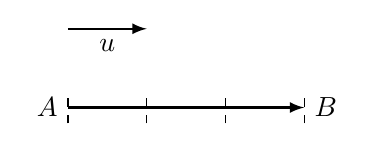
\begin{tikzpicture}
				\def\unidade{1cm}
				\draw[thick, -latex] (0,-1) coordinate (A) node[left] {$A$} -- (3*\unidade,-1) coordinate (B) node[right] {$B$};
				\foreach \i in {0,1,2,3} {
					\draw[dashed] (\i*\unidade,-1.2) -- (\i*\unidade,-0.8);
				}
				\draw[thick, -latex] (0,0) -- (\unidade,0) node[midway, below] {$u$};
			\end{tikzpicture}
			$|AB| = 3u$
			
		\subsection{Direção Entre Dois Segmentos Orientados}
			Sejam dois segmentos orientados $AB$ e $CD$. Dizemos que $AB$ tem a mesma direção de $CD$ se ambas as retas são \textbf{coincidentes} ou \textbf{paralelas}.\\
			
			
			\textbf{Coincidentes:}
			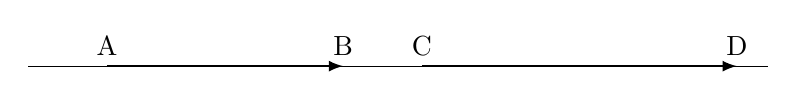
\begin{tikzpicture}
				\draw[thick,-latex](1,0) coordinate (A) node[above]{A} -- (4,0) coordinate (B) node[above]{B};
				\draw[thick,-latex](5,0) coordinate (C) node[above]{C} -- (9,0) coordinate (D) node[above]{D};
				\draw[thin](0,0) -- (9.4,0);
			\end{tikzpicture}
			\\
			
			
			\textbf{Paralelas:}
			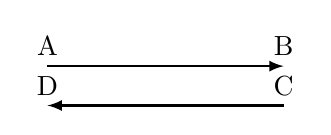
\begin{tikzpicture}
				\draw[thick,-latex](1,0) coordinate (A) node[above]{A} -- (4,0) coordinate (B) node[above]{B};
				\draw[thick,-latex](4,-0.5) coordinate (C) node[above]{C} -- (1,-0.5) coordinate (D) node[above]{D};
			\end{tikzpicture}
			
		\subsection{Sentido Entre Dois Segmentos Orientados}
			Dois segmentos orientados $AB$ e $CD$ \textbf{de mesma direção} podem ter o mesmo sentido ou sentidos opostos conforme abaixo:\\
			
			
			\textbf{Mesmo Sentido:}
			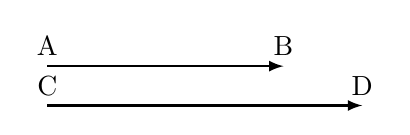
\begin{tikzpicture}
				\draw[thick,-latex](1,0) coordinate (A) node[above]{A} -- (4,0) coordinate (B) node[above]{B};
				\draw[thick,-latex](1,-0.5) coordinate (C) node[above]{C} -- (5,-0.5) coordinate (D) node[above]{D};
			\end{tikzpicture}\\
			

			\textbf{Sentidos Opostos:}
			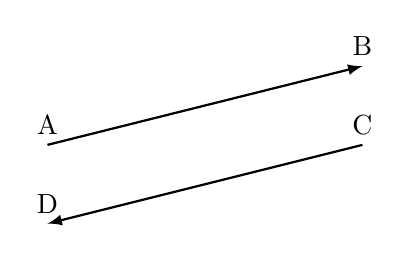
\begin{tikzpicture}
				\draw[thick,-latex](0,0) coordinate (A) node[above]{A} -- (4,1) coordinate (B) node[above]{B};
				\draw[thick,-latex](4,0) coordinate (C) node[above]{C} -- (0,-1) coordinate (D) node[above]{D};
			\end{tikzpicture}\\
		\subsection{Equipolência}
			Dois segmentos orientados são \textbf{equipolentes} se tiverem o mesmo \textbf{comprimento}, \textbf{direção} e \textbf{sentido}.\\
			Notação de equipolência: $AB \sim CD$\\
			\textbf{Propriedades de Segmentos Equipolentes:}
			\begin{itemize}
				\item \textbf{Reflexiva}: $AB \sim BA$.
				\item \textbf{Simétrica}: se $AB \sim CD$ então $BA \sim DC$.
				\item \textbf{Transitiva}: se $AB \sim CD$ e $CD \sim EF$ então $AB \sim EF$.
			\end{itemize}
			Dados um segmento orientado $AB$ e um ponto $C$, existe um único ponto $D$ tal que $AB \sim CD$.
			
	\section{Vetores}
		Sendo $AB$ um segmento orientado fixo, o vetor $AB$ é o conjunto de todos os segmentos orientados $CD$ tais que $CD \sim AB$.
		$$\overrightarrow{v} = AB = {CD,CD \sim AB}$$
		em que $AB$ é fixo.\\
		Dado um vetor $\overrightarrow{v}$ e um ponto $A$, por meio de seus representantes existe um único ponto $B$ tal que $A+ \overrightarrow{v} = B$.\\
		Notação $\overrightarrow{v} = B-A$
		\subsection{Igualdade de Vetores}
			Dizemos que dois vetores $AB$ e $CD$ são iguais quando $AB$ e $CD$ são equipolentes.\\
			\textbf{Propriedades de Vetores:}
			\begin{itemize}
				\item $A + \overrightarrow{o} = A$
				\item $A- \overrightarrow{v} = A + (-\overrightarrow{v})$
				\item $A+ \overrightarrow{v} = B + \overrightarrow{v} \to A=B$
				\item $A + \overrightarrow{v} = A + \overrightarrow{w} \to \overrightarrow{v} = \overrightarrow{w}$
				\item $A+(B-A)=B$
				\item $B-A = -(A-B)$
			\end{itemize}

		\subsection{Operações com Vetores: Adição}
			Dados os vetores $\overrightarrow{u}$ e $\overrightarrow{v}$, pelos seus representantes,conforme a figura abaixo:
			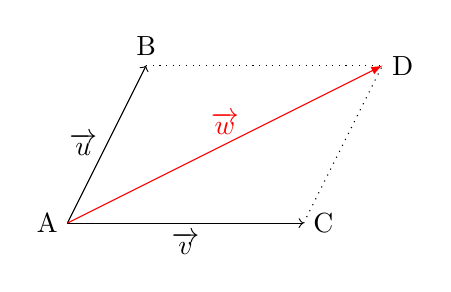
\begin{tikzpicture}
				\coordinate (A) at (0,0);
				\coordinate (B) at (1,2);
				\coordinate (C) at (3,0);
				\coordinate (D) at (4,2);
				
				\draw[->] (A) -- (B) node[midway, left] {$\overrightarrow{u}$};
				\draw[->] (A) -- (C) node[midway, below] {$\overrightarrow{v}$};
				\draw[dotted] (B) -- (D);
				\draw[dotted] (C) -- (D);
				\draw[->, red, -latex] (A) -- (D) node[midway, above]{$\overrightarrow{w}$};				
				
				\node at (A) [left] {A};
				\node at (B) [above] {B};
				\node at (C) [right] {C};
				\node at (D) [right] {D};
			\end{tikzpicture}
			$\overrightarrow{w}= \overrightarrow{u}+\overrightarrow{v}$, sendo $BD \sim AC$ e $AB \sim CD$
			\textbf{Propriedades da Soma de Vetores:}
			\begin{itemize}
				\item \textbf{Comutativa}: $\overrightarrow{u}+\overrightarrow{v}=\overrightarrow{v}+\overrightarrow{u}$
				\item \textbf{Associativa}: $(\overrightarrow{u}+\overrightarrow{v})+\overrightarrow{w}=\overrightarrow{u}+(\overrightarrow{v}+\overrightarrow{w})$
				\item \textbf{Elemento Neutro}: $\overrightarrow{u}+\overrightarrow{o} = \overrightarrow{u}$
				\item \textbf{Elemento Oposto}: Dado $\overrightarrow{u}$, existe um único $\overrightarrow{v}$ tal que $\overrightarrow{u}+\overrightarrow{v}=\overrightarrow{o}$, nesse caso $\overrightarrow{v}=- \overrightarrow{u}$
			\end{itemize}
			\begin{center}			
				Dados $\overrightarrow{u}$ e $\overrightarrow{v}$, temos que $\overrightarrow{u}-\overrightarrow{v}=\overrightarrow{u}+(-\overrightarrow{v})$\\
				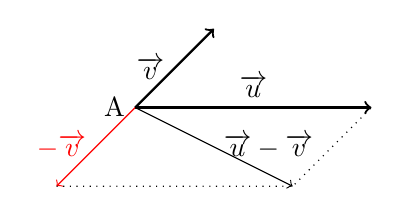
\begin{tikzpicture}
					\coordinate (A) at (0,0);
					\coordinate (v) at (1,1);
					\coordinate (-v) at (-1,-1);
					\coordinate (u) at (3,0);
					\coordinate (u-v) at (2,-1);
					
					\draw[->, thick] (A) node[left] {A} -- (u) node[midway, above] {$\overrightarrow{u}$};
					\draw[->,red] (A) -- (-v) node[midway,left]{$-\overrightarrow{v}$};
					\draw[->, thick] (A) -- (v) node[midway,left]{$\overrightarrow{v}$};
					\draw[->, thin] (A) -- (u-v) node[midway, right]{$\overrightarrow{u}-\overrightarrow{v}$};
					\draw[dotted] (-v) -- (u-v) -- (u);
				\end{tikzpicture}
			\end{center}
		\subsection{Operações com Vetores: Multiplicação de um Vetor por um Número Real}
			







		
		
		
		
		
	\newpage %A AULA QUE EU ESQUECI O CADERNO
	\section{Identidade de Lagrange}
		$$|u.v|^2 +(u.v)^2=|u|^2.|v|^2$$
		Com isso, temos:
		$$|u.v|^2=|u|^2.|v|^2-(u.v)^2$$
		Por outro lado,
		$$u.v=|u|.|v|.\cos(\theta)$$
		Substituindo a acima pela equação acima dela:
		$$|u.v|^2=|u|^2.|v|^2-(|u|.|v|.\cos(\theta))^2=|u|^2.|v|^2-|u|^2.|v|^.\cos^2(\theta)$$
		$$\to |u.v|^2 = |u|^2.|v|^2.(1-\cos^2(\theta))^2$$
		$$=|u|^2.|v|^2.\sin^2(\theta)$$
		
		Logo $|u.v|^2 = (|u|.|v|.\sin(\theta))^2$, se $0 \leq \theta \leq \pi$
		$$|u.v| = |u|.|v|.\sin(\theta)$$ %lagrange
		
		
		\subsection{Interpretação Geométrica}
			Pensando num paralelograma formado pelos vetores $v$ e $u$ e o ângulo $\theta$:
			%Imagem do paralelograma
			Área de um paralelograma é \textit{Base} x \textit{Altura}. Usando propriedades geométricas:
			$$h=|v|.\sin(\theta)$$
			Portanto, $A=b.h \to |u|.|v|.\sin(\theta)\to |u.v|$
			$$A=|u.v|$$%Área de um paralelogramo de dois vetores
			
			Exemplos:
			\begin{enumerate}
				\item Encontre a área do paralelogramo gerado pelos pontos:\\
				\begin{itemize}
					\item $A=(0,0,0)$
					\item $B=(2,0,0)$
					\item $C=(1,1,0)$
					\item $D=(3,1,0)$
$$				A=	\begin{vmatrix}
					       	i & j & k\\
						2 & 0 & 0\\
						1 & 1 & 0
					\end{vmatrix} $$
					$$=2.k$$
					$$= (0,0,2)$$
					$$|u.v| = \sqrt[]{0^2+0^2+2^2}$$
					$$A= 2$$%ua

				\end{itemize}
				\item Encontre a área do triângulo de vértice:\\
				\begin{itemize}
					\item $A=(1,1,0)$
					\item $B=(3,3,0)$
					\item $C=(2,4,0)$
				\end{itemize}
				Área de um triângulo é a metade da área de um paralelograma
				$$\overrightarrow{u}=\overrightarrow{AB}= B-A = (3,3,0)-(1,1,0)=(2,2,0)$$
				$$\overrightarrow{v}=\overrightarrow{AC} = C-A = (2,4,0)-(1,1,0)=(1,3,0)$$

				$$A = \begin{vmatrix}
					i&j&k\\
					2&2&0\\
					1&3&0
				\end{vmatrix}$$
				
				$$u.v=4k = (0,0,4)$$
				$$|u.v|=\sqrt[ ]{0^2+0^2+4^2}=4$$
				$$A = \dfrac{|u.v|}{2}=2$$
				\item Determine um vetor $\overrightarrow{x}$ tal que  $|x|=\sqrt[]{6}$ e $x.(i+k)=2.(i+j-k)$\\
				Seja $x = (a,b,c)$, então:
				$$a^2+b^2+c^2=6$$
				$$x.(i+k)=(a,b,c).((1,0,0)+(0,0,1)) = (a,b,c).(1,0,1)$$
				$$=\begin{vmatrix}
					i & j & k \\
					a &b &c\\
					1 &0 &1
				\end{vmatrix}$$
				$$=b.i+c.j-bk-aj=bi+(c-a)j-bk$$
				$$=2(i+j-k)$$
				$$=2i+2j-2k$$
				
				Logo $b=2$ e $c-a = 2$ ou $c=a+2$\\
				Considerando $a^2+b^2+c^2 = 6$:\\
				$$a^2+2^2+(a+2)^2=6$$
				$$a^2+4+a^2+4.a+4 = 6$$
				$$2.a^2+4.a+8 = 6$$
				$$a^2+2a+1=0$$
				$$(a+1)^2 = 0$$
				$$(a+1)=0$$
				Deste modo, $a=-1 , b=2 , c=1$
				\item Determine um vetor $\overrightarrow{u}$ tal que $|\overrightarrow{u}|=9$ e $\overrightarrow{u}$ é ortogonal a $\overrightarrow{v}= (1,2,1)$ e $\overrightarrow{w}(2,1,0)$
				Deste modo:
					$$|u|=9$$
					$$u \perp v$$
					$$u \perp w$$
					Para ser ortogonal a dois vetores, $u$ é um múltiplo de $v.w$.\\
					$$v.w = \begin{vmatrix}
						i &j&k\\
						1&2&1\\
						2&1&0
					\end{vmatrix}$$
					$$v.w=2j+k--4k-i= -i+2j-3k = (-1,2,-3)$$
					$$|v.w| = \sqrt[ ]{(-1)^2+(2)^2(-3)^2} = \sqrt[ ]{1+4+9}$$
					$$|v.w| = \sqrt[ ]{14}$$%Lembrar que esse . não é multiplicação, nas sim vxw (v vetorial w)
					Versor de  $v.w$ é dado como:
					$$\dfrac{1}{|v.w|}.(v.w)=\dfrac{1}{\sqrt[]{14}}.(-1,2,-3)=\overrightarrow{u}$$
					$$u= (\dfrac{-1}{\sqrt[ ]{14}}, \dfrac{2}{\sqrt[ ]{14}}, \dfrac{-3}{\sqrt[ ]{14}})$$
				Note que $\overrightarrow{u}$ tem a mesma direção e sentido de $\overrightarrow{v}.\overrightarrow{w}$ com $|\overrightarrow{u}|=1$
				$$\overrightarrow{x}=9.\overrightarrow{u} = 9.(\dfrac{-1}{\sqrt[ ]{14}}, \dfrac{2}{\sqrt[ ]{14}}, \dfrac{-3}{\sqrt[ ]{14}})$$
				$$\overrightarrow{x} = (\dfrac{-9}{\sqrt[ ]{14}}, \dfrac{18}{\sqrt[ ]{14}}, \dfrac{-27}{\sqrt[ ]{14}})$$
				$$|\overrightarrow{x}| = |9.\overrightarrow{u}|=9.1=9$$
			\end{enumerate}
	\section{Produto Misto}
	O produto misto serve para achar o volume de um paralelepípedo formado por 3 vetores.\\
	Sejam $\overrightarrow{u}$, $\overrightarrow{v}$ e $\overrightarrow{w}$ vetores. O produto misto de $\overrightarrow{u}$, $\overrightarrow{v}$ e $\overrightarrow{w}$ é definido por:
	$$[\overrightarrow{u},\overrightarrow{v},\overrightarrow{w}]= (\overrightarrow{u}.\overrightarrow{v}).\overrightarrow{w}$$
		\subsection{Interpretação Geométrica}
			%Imagem de um paralelepipedo determinado por 3 vetores, uma linha pontilhada determinando a altura h
			%página 100 do livro
			Pensando num paralelepipedo formado pelos vetores $\overrightarrow{u}$, $\overrightarrow{v}$ e $\overrightarrow{w}$. A área desse paralelepípedo é \textit{Área da Base} x \textit{Altura}. A base do paralelepípedo é o paralelogramo gerado pelos vetores $u$ e $ v$.\\
			Logo, \textit{Área da base} = $|u.v|$\\
			Por outro lado, temos :
			$$\cos(\Phi) = \dfrac{h}{|w|}$$
			$\Phi$ é o ângulo entre $|w|$ e $h$.
			Então $h=|w|\cos(\Phi)$, se $0 \leq \Phi \leq \dfrac{\pi}{2}$\\
			Daí, o volume $V = A.h = |u.v|.|w|.\cos(\Phi)$
			$$V=|(u.v).w|$$
			$$V= |[u,v,w]|$$
			Sabemos que $[u,v,w] =(u.v).w$. Sejam:
			\begin{itemize}
				\item $\overrightarrow{u} =(x_1,y_1,z_1)$
				\item $\overrightarrow{v} =(x_2,y_2,z_2)$
				\item $\overrightarrow{w}= (x_3,y_3,z_3)$
			\end{itemize}
			$$\overrightarrow{u}.\overrightarrow{v}= \begin{vmatrix}
			i&j&k\\
			x_1&y_1&z_1\\
			x_2&y_2&z_2
			\end{vmatrix}
			= i.(y_1.z_2-y_2.z_1)+j.(x_2.z_1-x_1.z_2)+k.(x_1.y_2-x_2.y_1)$$
			$$= i. \begin{vmatrix}
			y_1 & y_2\\
			z_1&z_2
			\end{vmatrix}
			+ j.
			\begin{vmatrix}
				x_2&x_1\\
				z_2&z_1
			\end{vmatrix}
			+k.
			\begin{vmatrix}
				x_1&x_2\\
				y_1&y_2
			\end{vmatrix}
			$$
			
			$$= (
			\begin{vmatrix}
			y_1 & y_2\\
			z_1&z_2
			\end{vmatrix}
			,
			\begin{vmatrix}
				x_2&x_1\\
				z_2&z_1
			\end{vmatrix}
			,
			\begin{vmatrix}
				x_1&x_2\\
				y_1&y_2
			\end{vmatrix}
			)$$			
		Logo, $[u,v,w] = (u.v).w$
		$$=(
			\begin{vmatrix}
			y_1 & y_2\\
			z_1&z_2
			\end{vmatrix}
			,
			\begin{vmatrix}
				x_2&x_1\\
				z_2&z_1
			\end{vmatrix}
			,
			\begin{vmatrix}
				x_1&x_2\\
				y_1&y_2
			\end{vmatrix}
			).
			(x_3,y_3,z_3)
		$$
		$$=
			x_3.
			\begin{vmatrix}
			y_1 & y_2\\
			z_1&z_2
			\end{vmatrix}
			+ y_3.
			\begin{vmatrix}
				x_2&x_1\\
				z_2&z_1
			\end{vmatrix}
			+z_3.
			\begin{vmatrix}
				x_1&x_2\\
				y_1&y_2
			\end{vmatrix}
			$$	
			Por outro lado, repare que:\\
					$$
					\begin{vmatrix}
						x_1 & y_1 & z_1\\
						x_2 & y_2 & z_2\\
						x_3 & y_3 & z_3
					\end{vmatrix}
					= (y_1.z_2-y_2.z_1).x_3 + (x_2.z_1-x_1.z_2).y_3+(x_1.y_2-x_2.y_1).z_3
					$$
			Logo, $ [u,v,w] = 
				\begin{vmatrix}
					x_1&y_1&z_1\\
					x_2&y_2&z_2\\
					x_3&y_3&z_3
				\end{vmatrix}						
			$ em que:
			\begin{itemize}
				\item $\overrightarrow{u} = (x_1,y_1,z_1)$
				\item $\overrightarrow{v} = (x_2,y_2,z_2)$
				\item $\overrightarrow{w} = (x_3,y_3,z_3)$
			\end{itemize}
		\subsection{Propriedades do Produto Misto}
			Tudo isso é comprovável manuseando os produto mistos usando o formato de determinantes.
			\begin{enumerate}
				\item Se $u$, $v$ e $w$ são linearmente dependentes, ou seja, exietem $ \alpha, \beta \in \mathbb{R}$; $w=\alpha.u + \beta.v$. Então $[u,v,w]=0$.
				\item $[u+u',v,w] = [u,v,w]+[u',v,w]$
				\item $[\alpha . u,v,w] = [u,\alpha .v, w] = [u,v, \alpha w]$
				\item $ [u,v,w] = -[u,w,v]=[v,w,u]=-[v,u,w]=[w,u,v]$ %Justificativas
			\end{enumerate}
			Explicando a primeira que é mais importante:
			$$[u,v,w]=[u,v,\alpha u +\beta v] = [u,v,\alpha u]+[u,v,\beta v]$$
			$$\alpha.[u,v,u]+\beta.[u,v,v]$$
			$$
				\alpha.
				\begin{vmatrix}
					x_1&y_1&z_1\\
					x_2&y_2&z_2\\
					x_1&y_1&z_1
				\end{vmatrix}		
				+ \beta
				\begin{vmatrix}
					x_1&y_1&z_1\\
					x_2&y_2&z_2\\
					x_2&y_2&z_2
				\end{vmatrix}								
			$$
			$$= \alpha . 0 + \beta.0$$
\end{document}